\subsubsection{ESP8266}

El \texttt{ESP8266} es un microcontrolador de bajo coste que dispone de conexión \texttt{Wi-Fi} integrada. Para programarlo, se utiliza \texttt{Arduino IDE}, programando en lenguaje \texttt{Arduino}.\cite{espressifsystemsESPRESSIFSMARTCONNECTIVITY}

En el sistema se utiliza para el monitoreo del sistema, gestión de medidas y control de los relés, así como para la conexión a la red \texttt{Wi-Fi} y el envío de las medidas a un servidor externo mediante el protocolo de comunicación \texttt{MQTT}.

\begin{figure}[h]
    \centering
    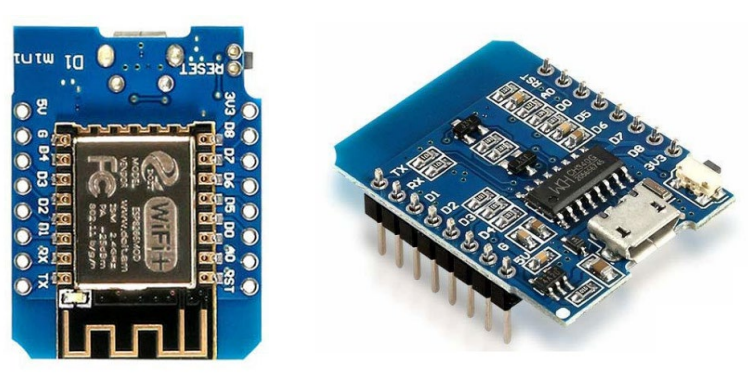
\includegraphics[width=0.5\textwidth]{images/2-hardware/componentes/ESP8266.png}
    \caption{\texttt{ESP8266}}
    \label{fig:hardware/modulos/esp8266}
\end{figure}

Se han utilizado los siguientes pines:

\begin{table}[H]
    \centering
    \begin{tabular}{l|c|c|}
    \cline{2-3}
                                                              & \textbf{Pin} & \textbf{GPIO} \\ \hline
    \multicolumn{1}{|l|}{\textbf{Relé para cargar la Backup}} & 7            & 13            \\ \hline
    \multicolumn{1}{|l|}{\textbf{Relé para la alimentación}}  & 8            & 15            \\ \hline
    \multicolumn{1}{|l|}{\textbf{SDA}}                        & 2            & 4             \\ \hline
    \multicolumn{1}{|l|}{\textbf{SCL}}                        & 1            & 5             \\ \hline
    \multicolumn{1}{|l|}{\textbf{Alimentación ESP8266}}       & 5V           & -             \\ \hline
    \multicolumn{1}{|l|}{\textbf{GND}}                        & GND          & -             \\ \hline
    \end{tabular}
\end{table}


\begin{figure}[h]
    \centering
    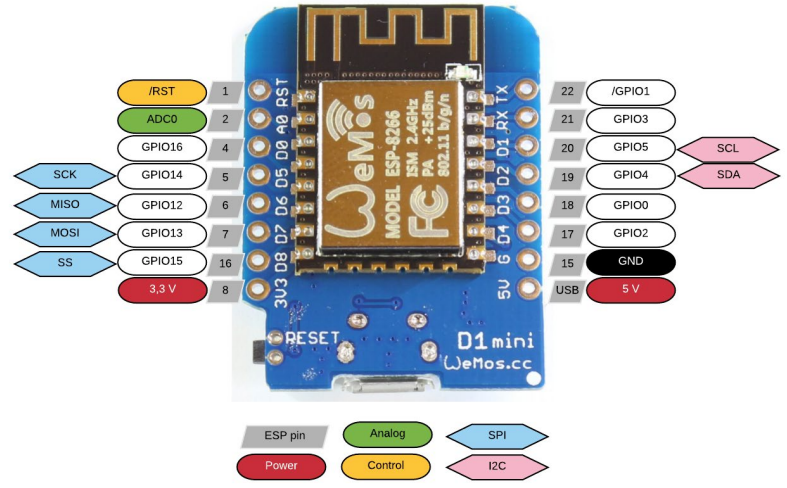
\includegraphics[width=0.7\textwidth]{images/2-hardware/componentes/conexiones_ESP.png}
    \caption{Conexiones \texttt{ESP8266}}
    \label{fig:hardware/modulos/conexiones_esp}
\end{figure}